\section{Front panel and headers}

		\begin{figure}[htbp!]
			\centering
			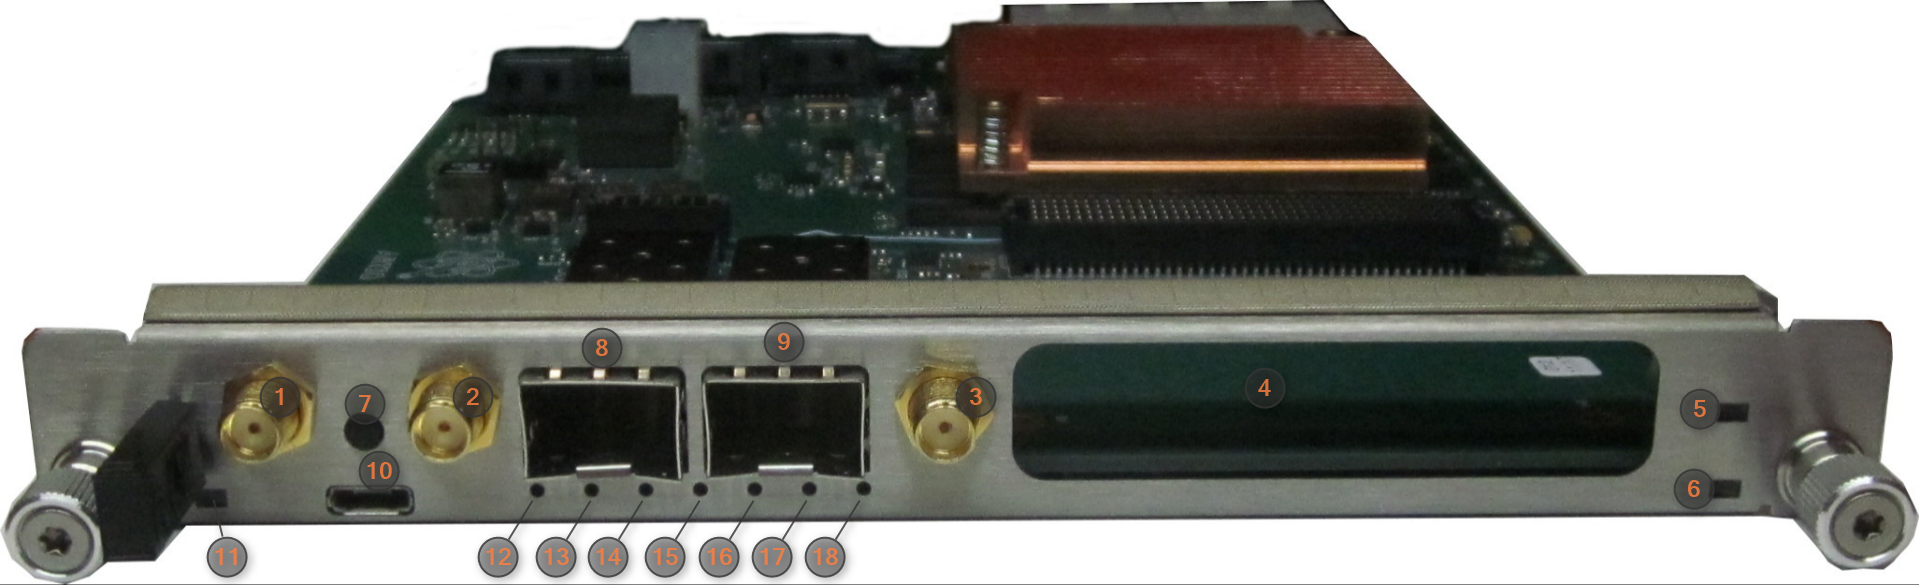
\includegraphics[width=14cm]{img/frontcallout.png}\\
			\caption{Front view}
		\end{figure}
		
		\begin{figure}[htbp!]
			\centering
			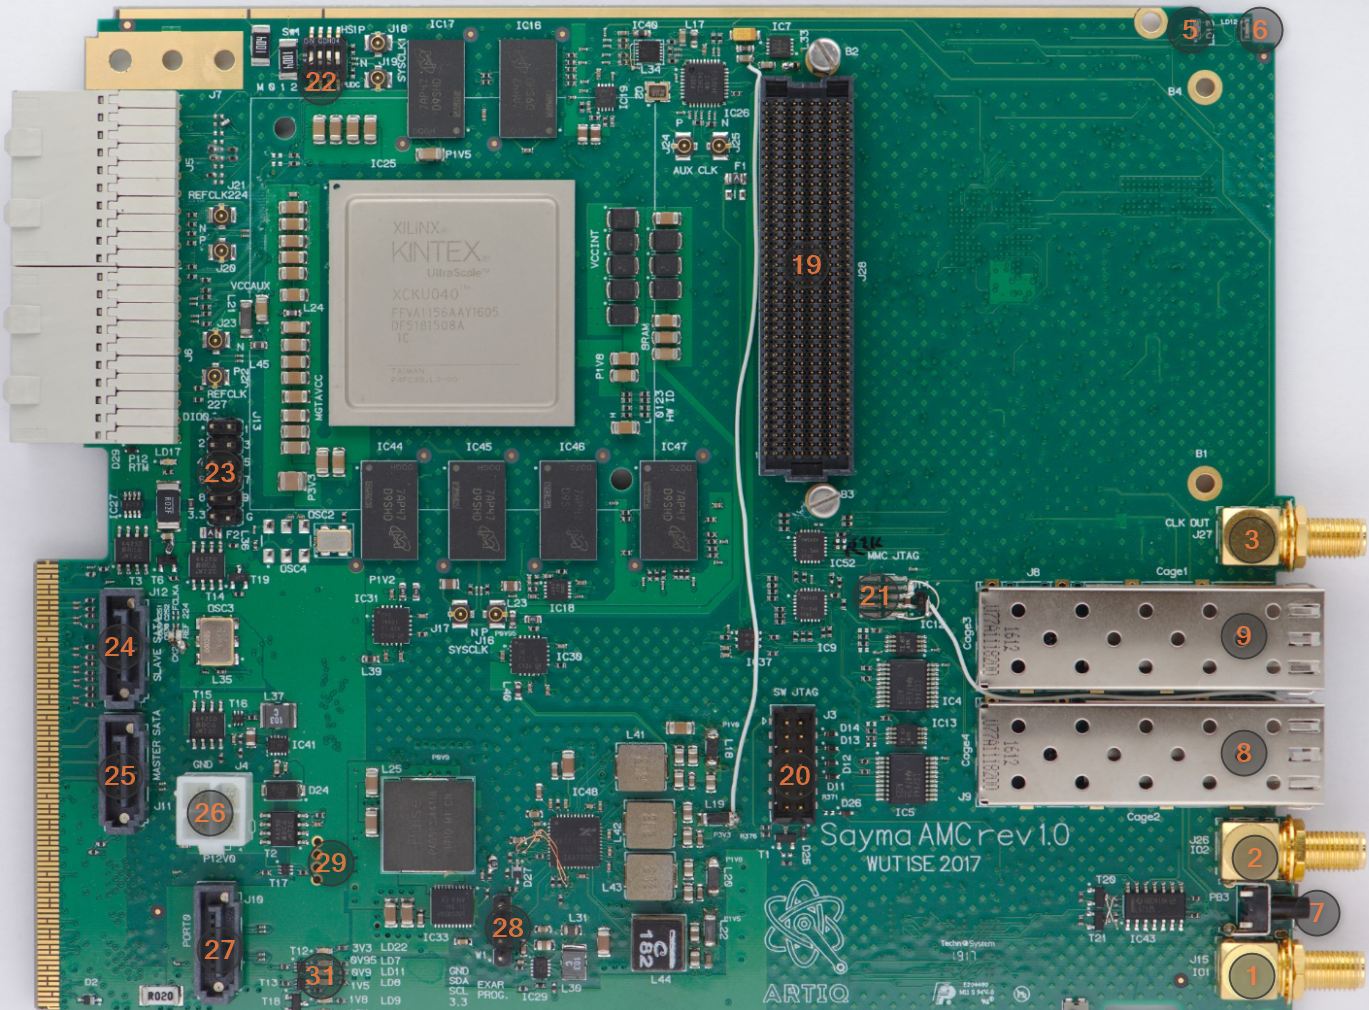
\includegraphics[width=14cm]{img/topcallout1.png}\\
			\caption{Front view}
		\end{figure}
\clearpage
		\begin{figure}[htbp!]
			\centering
			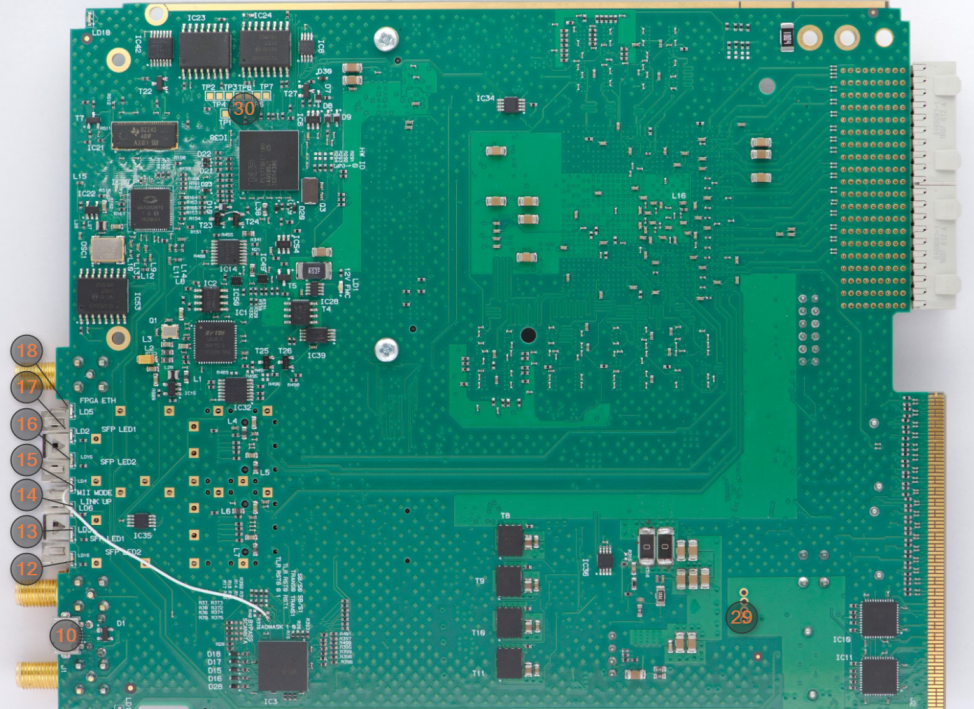
\includegraphics[width=14cm]{img/botcallout1.png}\\
			\caption{Front view}
		\end{figure}

\begin{longtable}{|c|c|c|} \hline
	\multicolumn{3}{|c|}{Call out table } \\ \hline	
	Call out & Designator & Description \\ \hline
	1 & J15 & IO1 \\ \hline
	2 & J26 & IO2 \\ \hline
	3 & J27 & CLK OUT \\ \hline
	4 & -- & FMC slot \\ \hline
%	5 & LD13 & Error\\ \hline
%	6 & LD18 & Hot swap \\ \hline
	7 & PB3 & reset? \\ \hline
	8 & cage2 & SFP Cage \\ \hline
	9 & cage1 & SFP Cage \\ \hline
	10 & J1 & Micro USB -->Serial \\ \hline
%	11& LD14 & operation successful  \\ \hline
%	12 & LD16 & SFP LED2 \\ \hline
%	13 & LD3 & SFP LED1 \\ \hline
%	14 & LD6 & LINK UP \\ \hline
%	15 & LD4 & MII MODE \\ \hline
%	16 & LD15 & SFP LED2  \\ \hline
%	17 & LD2 & SFP LED1 \\ \hline
%	18 & LD5 & FPGA ETH \\ \hline
	19 & J28 & FMC Header \\ \hline
	20 & J3 & SW JTAG \\ \hline
	21 & J14 & MMC JTAG \\ \hline
	22 & SW1 & FPGA MODE \\ \hline
	23 & J13 & Digital IOs \\ \hline
	24 & J12 & SLAVE SATA \\ \hline
	25 & J11 & MASTER SATA \\ \hline
	26 & J4 & Power In \\ \hline
	27 & J10 & Port 0 \\ \hline
	28 & W1 & EXAR I2C header \\ \hline
	29 & -- & P12V0 \\ \hline
	30 & -- &  Test points \\ \hline
\end{longtable}

\begin{longtable}{|c|c|c|c|c|c|c|} \hline
		\multicolumn{7}{|c|}{LED table }\\ \hline
	Call out & Designator & Description&  Colour &nominal state& IC &Failure\\ \hline
	5 & LD13 & Error &Red & off &MMC & on \\ \hline
	6 & LD4 & Hot Swap & Blue & on&  MMC &  off\\ \hline
	6 & LD21 & FPGA config done & Green & on& FPGA &off \\ \hline 
	11 & LD14 & Operation succesful& Green & on& MMC &off\\ \hline
	12 & LD3 & SFP2 LED2 & Red &on& FPGA & off\\ \hline
	13 & LD6 & SFP2 LED1 & Green &on & FPGA&off \\ \hline
	14 & LD20 & LINK UP &  Green &on & MAX24287&off \\ \hline
	15 & LD18 & MII MODE & Green & on& MMC&off \\ \hline
	16 & LD2 & SFP1 LED2 & Red & on& FPGA &off\\ \hline
	17& LD5 & SFP1 LED1 & Green &on & FPGA& off\\ \hline
	18 & LD19 & FPGA ETH & Green &on & MMC &off\\ \hline
	30 & LD22 & 3V3 & Green & on & Power & off \\ \hline
	30 & LD7 & 0V95 & Green & on & Power & off \\ \hline 
	30 & LD11 & 0V9 & Green & on & Power & off \\ \hline 
	30 & LD8 & 1V5 & Green & on & Power & off \\ \hline 
	30 & LD9 & 1V8 & Green & on & Power & off \\ \hline 
	30 & LD10 & 12V & Green & on & Power & off \\ \hline  
\end{longtable}

\subsection{Headers pinout}

		\begin{figure}[htbp!]
			\centering
			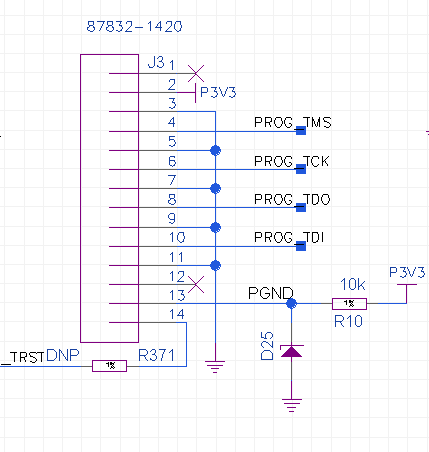
\includegraphics[width=9cm]{img/jtag1.png}\\
			\caption{JTAG - Call out 20}
		\end{figure}

		\begin{figure}[htbp!]
			\centering
			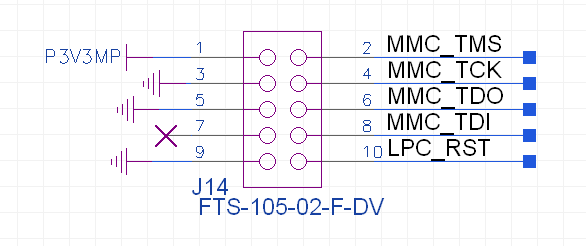
\includegraphics[width=9cm]{img/jtaglpc.png}\\
			\caption{JTAG - Call out  21}
		\end{figure}
		
		\begin{figure}[htbp!]
			\centering
			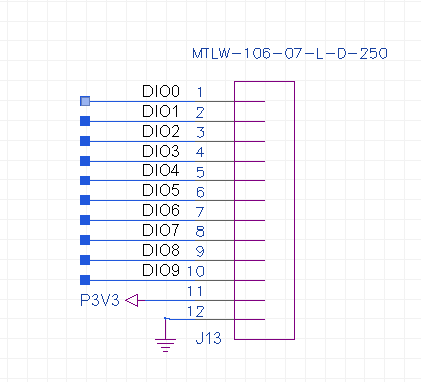
\includegraphics[width=9cm]{img/gpio.png}\\
			\caption{DIO - Call out 23}
		\end{figure}

\clearpage


\begin{longtable}{|c|c|c|} \hline
		\multicolumn{3}{|c|}{Tespoints table - Call out 30}\\ \hline
	TPx & Sig Name & LPC pin \\ \hline
	TP1 & MII1\_col & C13 \\ \hline
	TP2 & SDCLK & J10 \\ \hline
	TP3 & SDCMD & K14 \\ \hline
	TP4 & SDPWR & K11 \\ \hline
	TP5 & SDDAT0 & L14 \\ \hline
	TP6 & SDDAT1 & M12 \\ \hline
	TP7 & SDDAT2 & N14 \\ \hline
	TP8 & SDDAT3 & M11 \\ \hline
	
\end{longtable}	


\subsection{Location ICs}

		\begin{figure}[htbp!]
			\centering
			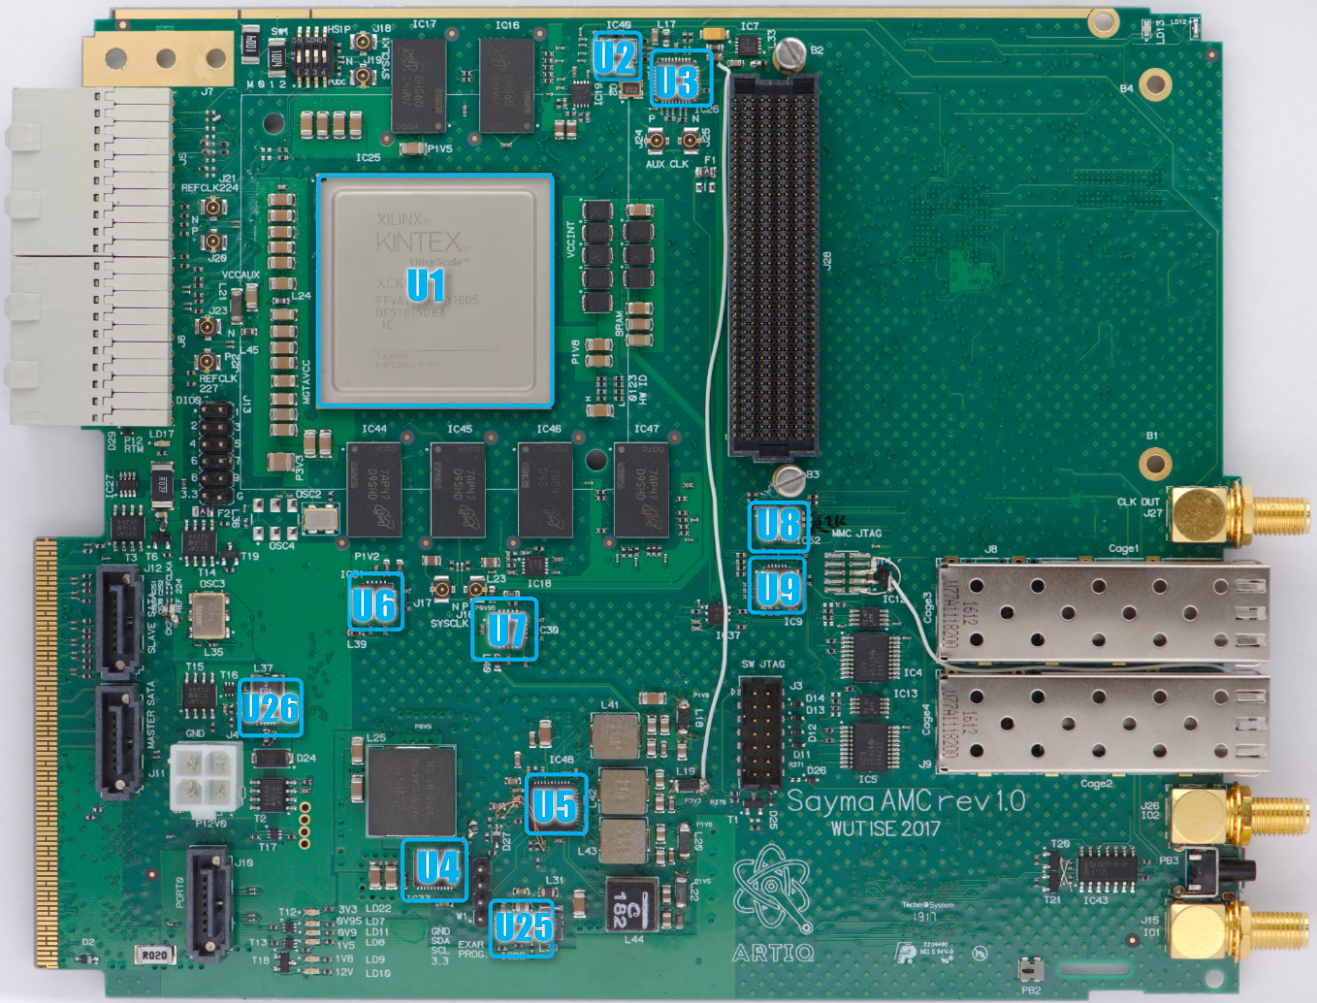
\includegraphics[width=14cm]{img/TU1.png}\\
			\caption{Top}
		\end{figure}
		\begin{figure}[htbp!]
			\centering
			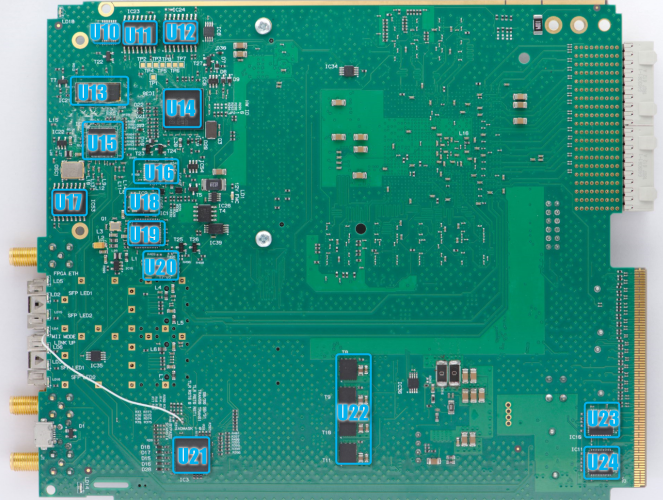
\includegraphics[width=14cm]{img/BU1.png}\\
			\caption{Bot}
		\end{figure}
\clearpage

\begin{longtable}{|c|c|c|} \hline
		\multicolumn{3}{|c|}{ICs Location}\\ \hline	
	Ux & IC & Description \\ \hline
	U1 & Kintex& FPGA \\ \hline
	U2 & LTC 6957&Low Phase Noise Buffer \\ \hline
	U4 & TPS53353  & P0V9\\ \hline
	U5 & XR77129 & EXAR\\ \hline
	U6 & TPS 74401  & P1V2\\ \hline
	U7 &  TPS 74401 & P0V95 \\ \hline
	U3 & SI5324C& Clock recovery \\ \hline
	U8 & TCA9548 &I2C switch - MMC\\ \hline
	U9 & TCA9548 &I2C switch - FPGA\\ \hline
	U10 & 74HC4066PW & Analog switch - Flash update\\ \hline
	U11 & N25Q256A13ESF40 & NOR Flash\\ \hline
	U12 & N25Q256A13ESF40 & NOR Flash\\ \hline
	U13 & SN74CB3Q32245ZKE  & Digital Bus switch - RGMI/MII\\ \hline
	U14 & LPC1776FET180  & MMC\\ \hline
	U15 & MAX24287ETK+ &ETH switch\\ \hline
	U16 & AN74CBT3257PW  & USB console switch\\ \hline
	U17 & N25Q256A13ESF40 & NOR Flash - MMC\\ \hline
	U18 & M93C46  & EEPROM\\ \hline
	U19 & F4232H-56Q & USB-UART Bridge \\ \hline
	U20 & 74HC4066PW & USB-UART Switch\\ \hline
	U21 & SCANSTA112SM & SCANSTA JTAG Switch\\ \hline
	U22 & FDMS7608S &EXAR Transistors \\ \hline
	U23 & SN65MLVD040RGZT &LVDS transceiver\\ \hline
	U24 & SN65MLVD040RGZT &LVDS transceiver \\ \hline
	U25 & TPS62175  & P5V0 \\ \hline
	U26 & TPS62175 & P3V3 \\ \hline
\end{longtable}


\subsection{SW1}

\begin{longtable}{|c|c|c|c|} \hline
			\multicolumn{4}{|c|}{SW1 table}\\ \hline
	M0 & M1 & M2 & Description \\ \hline
	0 & 0 & 0 & Master Serial Mode \\ \hline
	0 & 0 & 1 & Master Parallel Up \\ \hline
	0 & 1 & 1 & Master Parallel Down \\ \hline
	1 & 0 & 1 & Peripheral mode \\ \hline
	1 & 1 & 1 & Slave Serial mode \\ \hline
	
\end{longtable}	
